\documentclass[12pt]{amsart}
\usepackage[margin = 1in]{geometry}
\usepackage{amsmath, amssymb, amsthm, graphicx}
\usepackage{enumerate}
\usepackage[all]{xy}
\usepackage{mathrsfs}

%%%%%%%%%%%%%% COLOR COMMENTS! %%%%%%%%%%%%%%%
\usepackage{color}
\newcommand{\dzb}[1]{{\color{blue} \sf
    $\spadesuit\spadesuit\spadesuit$ DZB: [#1]}}
\newcommand{\reword}[1]{{\color{red} \sf $\spadesuit\spadesuit\spadesuit$ reword: [#1]}}

% changed above definition to make comments disappear
%\newcommand{dzb}[1]{}
%\newcommand{reword}[1]{}

% Color names: http://en.wikibooks.org/wiki/LaTeX/Colors#The_68_standard_colors_known_to_dvips
\usepackage[usenames,dvipsnames]{xcolor}
\newcommand{\note}[1]{{\color{BurntOrange} $\blacktriangle\blacktriangle$\sf Note: [#1]}}

\newcommand{\F}[0]{\mathbb{F}}
\newcommand{\tr}[0]{\operatorname{tr}}
\newcommand{\wt}[1]{\widetilde{#1}}
\newcommand{\frob}[0]{\operatorname{Frob}}
\newcommand{\card}[0]{\#}
\newcommand{\pmat}[4]{\begin{pmatrix}#1 & #2 \\ #3 & #4\end{pmatrix}}
\newcommand{\pderiv}[2]{\frac{\partial #1}{\partial #2}}
\newcommand{\Ov}{\mathcal{O}_{v}}
\newcommand{\Ok}{\mathcal{O}_{K}}
\newcommand{\Q}{\mathbb{Q}}
\newcommand{\Z}{\mathbb{Z}}
\newcommand{\C}{\mathbb{C}}
\newcommand{\leg}[2]{\left(\frac{#1}{#2}\right)}
\newcommand{\calO}{\mathcal{O}}
\newcommand{\frakp}{\mathfrak{p}}
\newcommand{\frakq}{\mathfrak{q}}
\newcommand{\mf}[1]{\mathfrak{#1}}
\newcommand{\nm}{\operatorname{N}_{K/\Q}}
\newcommand{\Cl}{\operatorname{Cl}}
\newcommand{\oo}{\mathcal{O}}
\newcommand{\sgn}{\operatorname{sgn}}
\newcommand{\Gal}{\operatorname{Gal}}
\newcommand{\cl}{\overline}
\newcommand{\mc}[1]{\mathcal{#1}}
\newcommand{\Cc}{\mathcal{C}}
\newcommand{\Dc}{\mathcal{D}}
\newcommand{\raym}{\mathcal{C}^{\frakm}_K}
\newcommand{\frakr}{\mathfrak{r}}
\newcommand{\Spec}{\text{Spec} \ }
\newcommand{\Hom}{\text{Hom}}
\newcommand{\ord}{\text{ord}}
\newcommand{\scr}[1]{\mathscr{#1}}
\newcommand{\R}{\mathbb{R}}
\newcommand{\cal}[1]{\mathcal{#1}}
\newcommand{\Nm}{\text{Nm}}
\newcommand{\A}{\mathbb{A}}
\newcommand{\ti}{\times}
\newcommand{\Hbb}{\mathbb{H}}
%\newcommand{\leg}[2]{\left(\frac{ \# 1}{\# 2} \right)}

\DeclareMathOperator{\GL}{GL}
\DeclareMathOperator{\SL}{SL}
\DeclareMathOperator{\Frob}{Frob}
\DeclareMathOperator{\ab}{ab}
\DeclareMathOperator{\cyc}{cyc}
\DeclareMathOperator{\N}{N}
\DeclareMathOperator{\Ver}{Ver}
\DeclareMathOperator{\Art}{Art}
\DeclareMathOperator{\Spl}{Spl}
\DeclareMathOperator{\sep}{sep}
\DeclareMathOperator{\Stab}{Stab}
\DeclareMathOperator{\Sp}{Sp}
\DeclareMathOperator{\SO}{SO}
\DeclareMathOperator{\SU}{SU}
\DeclareMathOperator{\PGL}{PGL}
\DeclareMathOperator{\Mat}{Mat}
\DeclareMathOperator{\Tr}{Tr}
\DeclareMathOperator{\End}{End}
\DeclareMathOperator{\Ad}{Ad}
\DeclareMathOperator{\Aut}{Aut}
\DeclareMathOperator{\WPr}{WPr}

\newtheorem{thm}{Theorem}
\newtheorem{lemma}[thm]{Lemma}
\newtheorem{defn}[thm]{Definition}
\newtheorem{prop}[thm]{Proposition}
\newtheorem{cor}[thm]{Corollary}
\newtheorem{ex}[thm]{Example}
\newtheorem{crit}[thm]{Criterion}


\theoremstyle{remark}
\newtheorem{rem}[thm]{Remark}

\makeatletter
\def\imod#1{\allowbreak\mkern5mu({\operator@font mod}\,\,#1)}
\makeatother

\widowpenalty=1000
\clubpenalty=1000

\title{CS 181 Problem Set 1}
\author{Ashok Cutkosky and Tony Feng}


\begin{document}
\maketitle

\noindent \textbf{Problem 1.} (a) We calculate respective information content of $A$ and $B$. First, we find the entropy of the variable. 
\[
H(X) = \left( \frac{4}{7} \log \frac{4}{7} + \frac{3}{7} \log \frac{3}{7} \right) \approx 0.985. 
\]
[This isn't actually necessary to determine which attribute has a higher information gain, unless they are equal and we are trying to determine if the gain is $0$.] 
\begin{itemize}
\item $A$ is true with probabiliy $\frac{4}{7}$, with a $2,2$ split, and false with probability $\frac{3}{7}$, with a $2,1$ split. Therefore, the conditional entropy of $A$ is 
\[
H(X \mid A) = - \left( \frac{4}{7} \left[ \frac{1}{2} \log \frac{1}{2} + \frac{1}{2} \log \frac{1}{2} \right] + 
\frac{3}{7} \left[ \frac{2}{3} \log \frac{2}{3} + \frac{1}{3} \log \frac{1}{3} \right] \right) \approx 0.965. 
\]
\item $B$ is true with probability $\frac{2}{7}$, with a $1,1$ split, and false with probability $\frac{5}{7}$, with a $3,2$-split. Therefore, 
\[
H(X \mid B) = - \left( \frac{2}{7} \left[ \frac{1}{2} \log \frac{1}{2} + \frac{1}{2} \log \frac{1}{2} \right]  + \frac{5}{7} \left[ \frac{3}{5} \log \frac{3}{5} + \frac{2}{5} \log \frac{2}{5} \right] \right) \approx 0.980.
\]
\end{itemize} 
Therefore, $I(X,A) = H(X) - H(X \mid A) \geq H(X) - H(X \mid B) = I(X,B)$. We conclude that $A$ gives a higher information gain. 

The differences and datasets are so small that it is difficult to give a convincing argument either way. The 
$2,1$ split when $A$ is false perhaps suggests that it is a good indicator, but the sample size is just too 
small to be decisive. Furthermore, it appears that $B$ does not split the data as well as $A$: its tree is more 
lopsided. A case for $B$ could be mode with the observation that the $2,2$ split when $A$ is true suggests 
that it is a poor indicator; the $1,1$ split for $B$ true is more noisy. 

The example demonstrates that ID3's inductive bias that objects can classified by sequential splitting on features one-by-one, unmindful of more ``forward-looking'' connections, can be flimsy in practice. \\

(b)  Note that $C$ and $D$ have the exact same description of $B$, in terms of how many objects fell into each value of the attribute, and the distribution of classifications of each objects (in particular, each have one positive and one negative for some value of the attribute, and three positive and two negative for the other). Therefore, the calculation we did in (a) demonstrates that $A$ has the highest information gain. 

When $A$ is true, the subdata obtained is 
\[
\begin{tabular}{lll|l}
\hline
B & C & D & Label \\
\hline
0 & 1 & 0 & 0 \\
0 & 0 & 0 & 1 \\
0 & 0 & 1 & 1 \\
1 & 0 & 1 & 0 \\
\hline
\end{tabular}
\]
Now $B$ and $C$ have identical classification results: one negative when $1$, two positive and one negative when $0$. On the other hand $D$ evidently has zero mutual information: there is one negative and one positive in either case. Therefore, $B$ and $C$ clearly have equal mutual information with $X$, higher than $D$'s, and we split on $B$ by alphabetical order. At this point, the subdata is 
When $A$ is true, the subtree obtained is 
\[
\begin{tabular}{ll|l}
\hline
 C & D & Label \\
\hline
1 & 0 & 0 \\
 0 & 0 & 1 \\
 0 & 1 & 1 \\
\end{tabular}
\]
Now $C$ perfectly classifies the data. To summarize, the left half of the tree we built is:
\[
\xymatrix{
 & &  &  & A \ar[dll]^1& & & &  \\
& &  \ar[dll]^1 B \ar[dr]^0  & & & & &\\
0&  & &  C \ar[dl]^0 \ar[dr]^1 &   & & & & \\
 & & 1 & & 0 &  & & & 
}
\]
For the right half, the subdata is 
\[
\begin{tabular}{lll|l}
\hline
B & C & D & Label \\
\hline
0 & 0 & 1 & 0 \\
0 & 1 & 1 & 1 \\
0 & 0 & 1 & 1 \\
\hline
\end{tabular}
\]
All examples have the same value for $B$ and $D$, so clearly $B$ and $D$ offer no information whatsoever! Splitting on $C$, we find that there are two identical, inconsistent examples left, evenly split between $0$ and $1$. We arbitrarily choose to classify them as $1$. 
\[
\xymatrix{
 & &  &  & A \ar[dll]^0 \ar[drr]^1& & & &  \\
& &  \ar[dll]^1 B \ar[dr]^0  & & & & C \ar[dl]^0 \ar[dr]^1&\\
0&  & &  C \ar[dl]^0 \ar[dr]^1 &   & 0& & 1&\\
 & & 1 & & 0 &  & & & 
}
\]

(c) Obviously, no tree can classify all examples since there are two inconsistent ones. However, some inspection shows that not($B$ xor $C$) classifies all but the third example, 0 0 0 1 | 0. 
\[
\xymatrix{
& & & \ar[dll]^1 \ar[drr]^0 B  & & & \\
& C \ar[dl]^1 \ar[dr]^0 & & & & C \ar[dl]^1 \ar[dr]^0 \\
1 & & 0 & & 0 &  & 1
}
\]

\newpage

\noindent \textbf{Problem 2.} (a) For the non-noisy dataset, we found a training performance of $1.0$ and a test performance of $0.87$. For the noisy dataset, we found a training performance of $0.98$ and a test performance of $0.78$. 

(b) See the graphs below, depicting the results with and without randomization of the validation set. Note that the learning scores here include \emph{both} the training data and data used for testing. (Obviously, the performance on training data will tend to $1$ as the training data tends to size zero, so that is uninteresting.) 


\begin{figure}[!h]
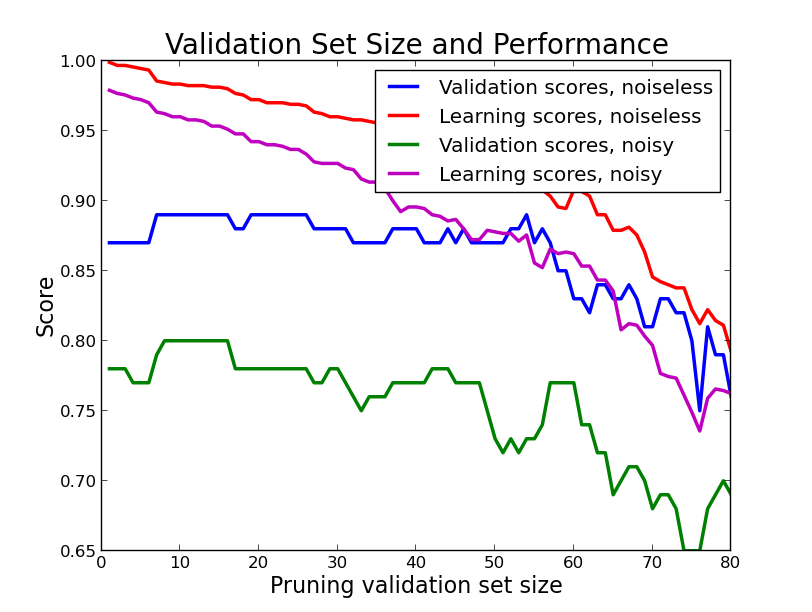
\includegraphics[scale=.4]{pruneperformancenorandom.png}
\caption{Without randomization}
\end{figure}

\begin{figure}[!h]
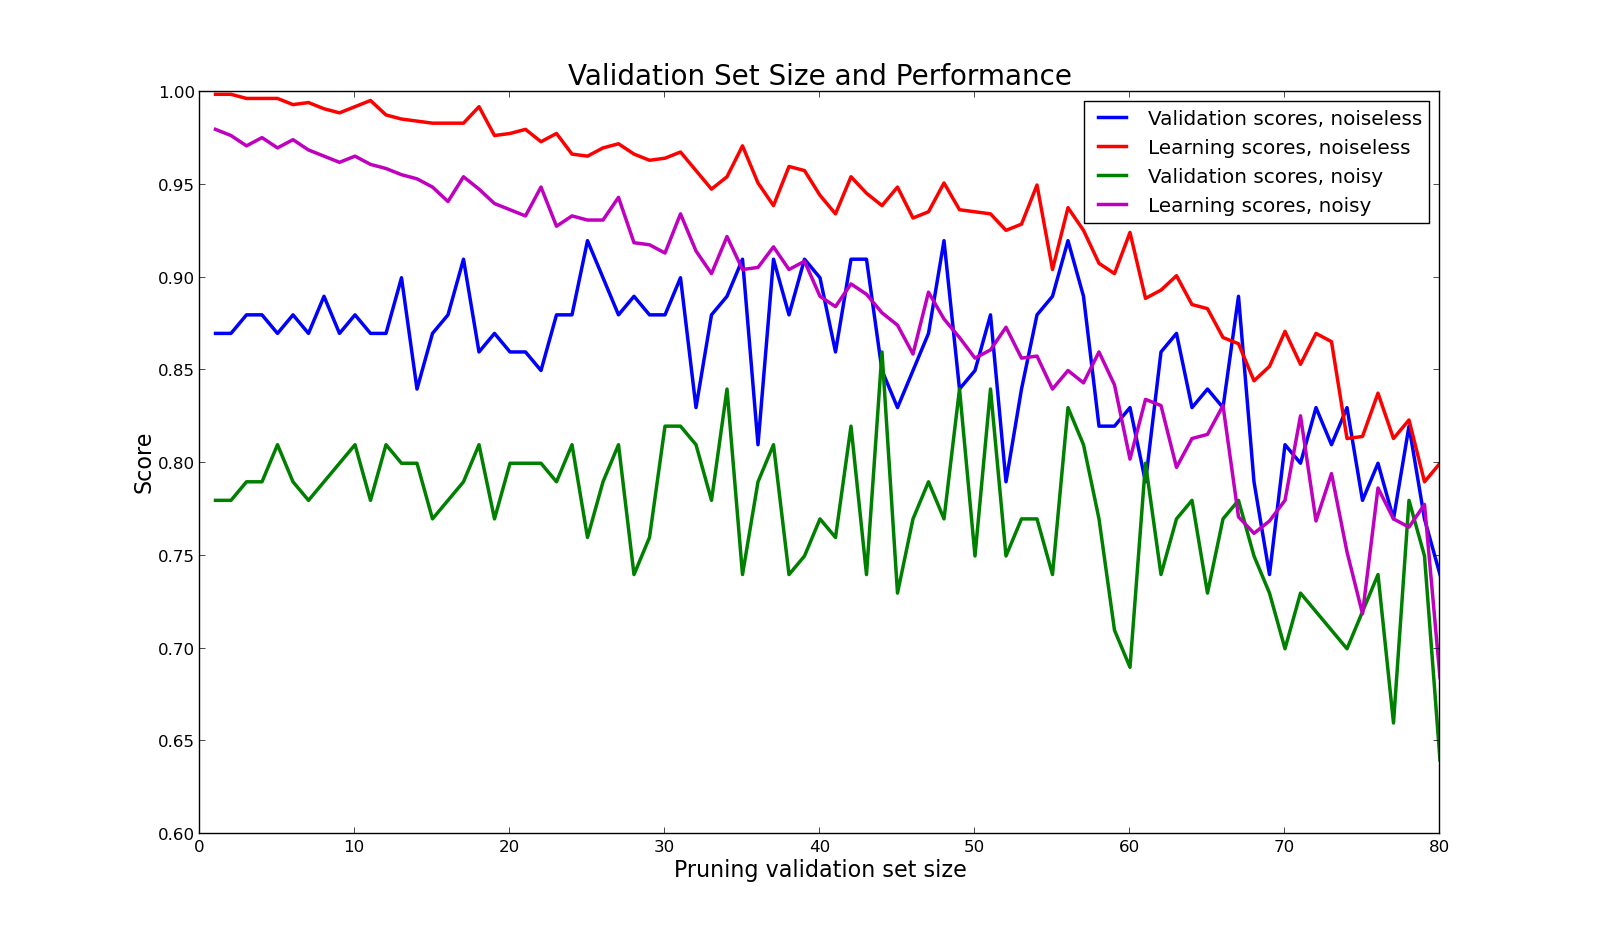
\includegraphics[scale=.4]{pruneperformance.png}
\caption{With randomization}
\end{figure}



(c) Validation set pruning does improve performance. In both cases, the test performance increased initially with validation set size and eventually dipped back down. This is to be expected: when the validation set is too large, there is not enough training data. To speak to the details of each scenario:

\begin{itemize}
\item Without randomization, the test performance increases from $0.78$ up to $0.80$ (peaking at a size between $10$ and $20$, and then dips back down. The trend is relatively stable. 
\item With randomization, the test performance is much less stable, but it peaks at around $0.86$ between $40$ and $50$ (but the worst performance also decreases steadily). 
\end{itemize}

(d) The results do seem indicate some level of overfitting. First, the fact that pruning improves performance suggests that the trees obtained without pruning are too complex, which corresponds to overfitting. Furthermore, validation test performance improves even while the performance on the learning set decreases, which is another indication that the trees being constructed with no validation pruning are overfitted to the training data. 
\newpage

\noindent \textbf{Problem 3.} (a)  Let $w(x_i)$ be the weight of $x_i$. We define the \emph{weighted} mass function of the examples $x_1, \ldots, x_n$ by 
\[
M = \sum_{i=1}^n w(x_i). 
\]
Scaling the weighting, we may assume that $M=1$. Then introduce the idea of weighted entropy by replacing each discrete example $x_i$ with a probability mass of size $w(x_i)$. Formally, if $X$ represents the classification and $\Omega$ its values, then we define the weighted probability 
\[
Pr_w(\omega) = \sum_{X(x_i) = \omega} w(x_i) 
\]
The weighted information is $I_w(\omega)  := \log \frac{1}{Pr_w(\omega)}$, and the weighted entropy is 
\[
H_w(X) = \sum_{\omega \in \Omega} Pr_w(\omega) I_w(\omega)
\]
If $y$ is a value of the random variable $Y$, then we extend this definition 
\[
Pr_w(y) = \sum_{Y(x_i) = y} w(x_i).
\]
Analogously, the weighted conditional probability is 
\[
Pr_w(\omega \mid y) =\frac{ \sum_{X(x_i) = \omega, Y(x_i) = y} w(x_i)}{Pr_w(y)}
\]
and the weighted conditional information is $I_w(\omega \mid y ) := \log \frac{1}{Pr_w(\omega \mid y)}$. 
Finally we define the weighted conditional entropy to be  
\[
H_w(X \mid Y) = \sum_y Pr_w(y) \sum_{\omega \in \Omega} Pr_w(\omega \mid y) I_w(\omega \mid y).
\]
As mentioned above, this is the ordinary entropy obtained by viewing each $x_i$ as representing a proportion $w(x_i)$ of the data, which is a reasonable interpretation of weighting (but how well this works obviously depends on how the weighting is constructed). 

\textbf{A.} 
\[
\begin{tabular}{|l|l|l|l|}
\hline
 Rounds & 10 & 30 \\
\hline
Depth 1& 0.93 &  0.94 \\
Depth 2 & 0.94 &  0.87\\
\hline
\end{tabular}
\]

\textbf{C.} Boosting appears to beat the ID3 algorithm, both with and without pruning, by a significant margin. \\

\textbf{D.} The performance on validation and training data are, respectively:

\paragraph{Validation.}  [0.88, 0.87, 0.9, 0.9, 0.92, 0.91, 0.93, 0.92, 0.94, 0.93, 0.92, 0.93, 0.93, 0.93, 0.93]\\
 

\paragraph{Training.} [0.953, 0.931, 0.989, 0.992, 0.997, 0.999, 1.0, 1.0, 1.0, 1.0, 1.0, 1.0, 1.0, 1.0, 1.0]

The validation improves with the training. This suggests that boosting is not overfitting (in contrast to our argument for overfitting in Problem 2). 

\newpage

\noindent \textbf{Problem 4.} 
\end{document}



